\chapter{Web Applikationen}

Der Titel dieses Dokumentes ist Web Security, dementsprechend sind unsere Zeile/Patienten auch Webapplikationen. Eine Definition fällt nicht einfach --- allgemein betrachtet ist eine Webapplikation eine auf der Client-Server-Architektur basierte Applikation die als Kommunikationsprotokoll HTTP verwendet.

Bei einer Client-Server Applikation versendet der Client einen Auftrag an einen Server; letzterer führt den Auftrag im Namen des Clients aus und sendet die Antwort zurück. Wir betrachten immer die Gesamtkonstellation von Client (Webbrowser) und Server.

Aktuell ist HTTP 1.0/1.1 im Desktop-Bereich die häufigst verwendete HTTP Version, im Mobilbereich wird gerne HTTP/2 eingesetzt. Aktuell (2019) wird an der Spezifikation von HTTP/3.0 gearbeitet.

\section{Struktur}

Eine Webapplikation besitzt sowohl eine interne Architektur (Struktur der Applikation bzw. des Source Codes) als auch eine Systemarchitektur (Integration mit externen Systemen). Eine Webapplikation wird in einer oder mehreren Programmiersprachen implementiert, zumeist unter Zuhilfenahme von Web-Frameworks bzw. -bibliotheken (diese können auch Bestandteil der Standardbibliothek einer der verwendeten Programmiersprachen sein).

Das Werk des Entwicklers ist der Source Code, welcher die benötigten Funktionen der Webapplikation implementiert. In Abhängigkeit von der verwendeten Technologie wird dieser Code auf den Applikationsserver als source code oder in kompilierter Form eingespielt und auf diesem schlußendlich auch exekutiert. Während der Exekution wird zumeist ein Applikationsserver involviert. Dieser kann entweder als eigenständiger Prozess (z. B. \textit{Apache Tomcat} als Applikationsserver für Java Servlets), innerhalb des Webservers (z. B. die Kombination von Apache Webserver mit \textit{mod\_php} für PHP) oder sogar ein Teil des kompilierten Programms sein (z. B. bei Verwendung von statischen binaries mit Go oder Rust).

Ein häufiges Problem ist die Zuordnung der Admin-Verantwortung zu den jeweiligen Komponenten. Es kann passieren, dass Entwickler davon ausgehen, dass eine Komponente von Administratoren verwaltet wird und vice versa. Dadurch kann es zum Unterlassen wichtiger Updates kommen.

\subsection{Wahl der Programmiersprache}

Zur Umsetzung einer Applikation wird eine Programmiersprache bemüht. Je nach Abstraktionslevel und Zielpublikum der Programmiersprache (bzw. des verwendeten Frameworks) ergeben sich positive und negative Auswirkungen auf die Sicherheit der Applikation.

Hierdurch sollte allerdings kein Chauvinismus bedingt werden. Es ist sowohl möglich in einer sicheren Programmiersprache unsicher zu programmieren als auch vice versa. Programmierer sollten sich der jeweiligen Eigenarten der gewählten Programmiersprache bewußt sein und ggf. vorsorglich gewisse Features nur unter Bedacht einsetzen.

Einflussreicher auf die Sicherheit der Applikation ist die Selektion von sicheren Bibliotheken und Komponenten. Hier sollten Komponenten mit einer guten Sicherheitshistorie gewählt werden, es ist essentiell, zeitnahe auch Sicherheitsupdates für verwendete Komponenten einzuspielen.

\subsection{Interne Architektur}

Die interne Struktur beschreibt, wie die Webapplikation selbst gebaut und der Code strukturiert wurde --- wie die Funtkionen auf Source-Code Komponenten aufgeteilt wurden. Die interne Architektur wird stark durch das verwendete Framework und der verwendeten Programmiersprache geprägt. Es ist sinnvoll, sich an die Annahmen und Konventionen des verwendeten Frameworks zu halten anstatt gegen diese Konventionen anzukämpfen.

\subsubsection{Request-Routing}

Ein guter Unterscheidungspunkt ist, wie der Webserver erkennen kann, dass ein eingehender HTTP Request über einen Applikationsserver, und damit als Applikationscode, ausgeführt werden soll. Initial wurde dies primär über die Dateien im Dateisystem erkannt. Gegeben ein Webroot von \url{/var/www/} und eine Datei \url{/var/www/operation.php} wird ein Aufruf der zugeordneten Webseite \url{https://www.example.local/operation.php} an die Datei \textit{operation.php} weitergeleitet und (falls PHP am server konfiguriert wurde) als PHP Applikation ausgeführt. Dieser Aufbau ist fehleranfällig: falls ein Entwickler eine .php-Datei am Server vergisst oder ein Angreifer eine zusätzliche .php-Datei am Server hochladen kann, kann es zu einer ungewollten Code-Execution kommen. Neuere Frameworks bieten zumeist die Möglichkeit, ein explizites Request-Routing zu definieren, so könnte z. B. das PHP-Framework Laraval mit folgender \url{routes/web.php} Konfiguration\footnote{\url{https://laravel.com/docs/5.7/routing}} gestartet werden:

\begin{minted}{php}
Route::get('/operation.php', 'SomeController@operation');
\end{minted}

In diesem Fall wird ein eingehender Request auf \url{/operation.php} an die Methode \textit{operation} des Controllers \textit{SomeController} weitergeleitet. Auf diese Weise wird explizit definiert, welche Operationen wie erreichbar sind und wo sich der aufzurufende Source-Code befindet.

\subsubsection{Model-View-Controller (MVC) Pattern}

Ein häufiges Muster für die interne Code-Struktur ist das MVC-Pattern. Hier wird die Funktionalität auf folgende groben Bereiche aufgeteilt:

\begin{description}
	\item[Model] ist zuständig für die Speicherung von Daten. Zumeist wird die Geschäftslogik innerhalb des Models abgebildet (\textit{thin controller, fat model}).
	\item[View]: eine View dient zur Darstellung von Daten. Zumeist wird jede einzelne Webseite über ein View-Objekt abgebildet. Mehrere View-Objekte pro Datum sind möglich, so kann z. B. das gleiche Model mittels einer View als Webseite ausgegeben ausgegeben, und mittels eines weiteren View-Objekts als Excel-Sheet heruntergeladen, werden.
	\item[Controller] akzeptiert Eingaben (z. B. HTTP- oder WebSocket-Requests), überprüft diese und interagiert mit dem Model um Geschäftsprozesse anzustossen. Um eine Antwort gegenüber dem Client zu präsentieren, werden Daten vom Controller an die View-Objekte übergeben.
\end{description}

Klassische Webapplikationen waren historisch thin-client Applikationen: die gesamte Logik wird server-seitig ausgeführt, der Client (Webbrowser) dient rein zur statischen Darstellung. Mit JavaScript entstand die Möglichkeit, innerhalb des Browsers Code auszuführen. Einige Frameworks wie \textit{Angular.js} implementieren das MVC-Pattern samt Routing innerhalb des Browsers. Der Server dient als Datenquelle und bietet jene zumeist über Webservices an.

Die Wahl der Struktur besitzt Einfluss auf Sicherheitsentscheidungen der Applikation. Bei einem klasssischen server-seitigen MVC-Pattern werden z. B. technische Überprüfungen auf Schadcode in User-Eingaben, Authentication- und Authorization-Checks innerhalb von Controllern implementiert. Wird client-seitig JavaScript verwendet, muss der server-seitige Service eine Überprüfung der JavaScript-Anfragen auf Schadcode, Authentication- und Authorization durchführen.

\subsubsection{Single-Page Applications und Progressive Web Applications}

Die Möglichkeiten von JavaScript und HTML5 wurden immer mächtiger. Dies führte zu Architekturen wie Single-Page Applications (SPA) bei denen alle Inhalte dynamisch per JavaScript geladen bzw. generiert werden. Werden diese SPAs mit HTML5 Offline-Fähigkeiten (HTML5 localStorage) und langlebigen nebenläufigen JavaScript-Prozessen (HTML5 WebWorker) kombiniert, könnnen offline lauffähige Webseiten geschrieben werden, die klassischen Desktop-Applikationen  sehr ähnlich sind. Diese werden häufig Progressive Web Applications (PWA) genannt. Werden Daten offline gespeichert, müssen deren Integrität und Vertraulichkeit mit geeigneten Methoden gewährleistet werden.

\subsection{System-Architektur einer primitiven Web-Applikation}

Eine einfache Webapplikation wird zumeist aus drei groben Komponenten bestehen:

\begin{itemize}
	\item Webserver: dient zur Bereitstellung statischer Dateien und leitet dynamische Anfragen an die jeweiligen Applikationsserver weiter. Webserver sind optimiert für das effiziente Zustellen statischer Inhalte.
	\item Applikationsserver: beinhalten die Applikation und bieten die Laufzeitumgebung der Applikation an. Die Applikation kommuniziert mit einer Datenbank zur Speicherung dynamischer Daten.
	\item Datenbank: beinhaltet dynamische Daten.
\end{itemize}

Die Bearbeitung einer Client-Anfrage durch den Applikationsserver kann längere Zeit benötigen. Während der Bearbeitung blockiert der Applikationsserver --- um einen höheren Durchsatz und geringere Latenzzeiten zu erreichen wird häufig ein Webserver mit mehreren Applikationsservern kombiniert.

Je nach Webserver- und Applikationsserverimplementierung kann der Applikationsserver Teil des Webservers sein. Intern sind die Funktionalitäten allerdings getrennt. Im Sinne von Separation of Concerns ist es vorteilhaft, Applikationsserver und Webserver zu trennen. Dadurch ist es möglich, die unterschiedlichen Serverprozesse mit eigenständigen Benutzerrollen zu betreiben.

\subsubsection{Potentielle zusätzliche Komponenten bei Webapplikationen}

Während Webserver, Applikationsserver und Datenbank zum Betrieb einer dynamischen Webapplikation prinzipiell ausreichen, kann es zu einer Inflation von externen Komponenten kommen:

\begin{figure}[h!]
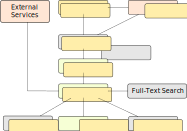
\includegraphics[width=10cm]{images/web_components.pdf}
\centering
\end{figure}

Um einige der hier vorkommenden Komponenten zu erwähnen:

\begin{itemize}
	\item Load-Balancer: verteilen den Traffic auf mehrere Webserver. Hier kann es zu Problemen beim Session-Management kommen.
	\item Content Delivery Networks (CDNs): dienen zur Performancesteigerung bei der Zustellung statischer Daten. Die Inhalte werden über ein geographisch verteiltes Netzwerk direkt an die Clients zugestellt.
	\item Caching Services werden verwendet, um häufig benötigte Daten oder Webseitenfragmente zwischenzuspeichern. Zumeist geschieht dies in-memory, bekannte Produkte sind z. B. memcached. Ein häufiges Problem ist, dass der Zugriff ohne Überprüfung der Authorisierung erfolgt. Somit erhält ein Angreifer mit Zugriff auf einen Caching Service potentiell auch Zugriff auf sensible Daten.
	\item Job Server: eine Client-Anfrage muss innerhalb kurzer Zeit beantwortet werden, falls dies nicht erfolgt kann im worst-case der Client-Browser die Verbindung unterbrechen. Um trotzdem langfristige Operationen auszuführen, können diese nebenläufig durch einen Job-Servers ausgeführt werden. Bekannte Produkte in diesem Umfeld sind RabbitMQ oder Redis. Ein potentielles Problem ist, dass Jobs Datenbankzugriffe benötigen und daher der Job Worker eine bestehende Verbindung zur Datenbank besitzt (welche von einem Angreifer ausgenutzt werden kann).
	\item Full-Text Search: viele Webapplikationen benötigen eine Volltextsuche, diese wird teilweise über einen externen Suchserver implementiert. Dieser beinhaltet eine bearbeite Version des Datenbestands der Datenbank. Ein mögliches Problem sind fehlende Berechtigungsüberprüfungen --- während auf der Datenbank der Datenzugriff zwar eingeschränkt wird, wird dies häufig innerhalb der Suchdatenbank vergessen.
	\item External Services werden häufig von Webapplikationen aufgerufen bzw. integriert. Ein Problem dabei ist, dass Webapplikationen häufig davon ausgehen, dass externe Services sich an definierte Protokolle halten.
\end{itemize}

\section{Angriffsfläche/Attack Surface}

Die Angriffsfläche ist jener Bereich, auf den ein potentieller Angreifer Zugriff erhält. Die extern sichtbare Webapplikation ist Teil der Angriffsfläche. Im Sinne der Systemsicherheit sollten Entwickler versuchen, die Angriffsfläche zu minimieren. Problematisch ist, dass die Angriffsfläche nicht nur die direkte Applikation, sondern auch alle verbundenen Funktionen und Komponenten, beinhaltet. Bei der Definition der Angriffsfläche sollten u.a. folgende Fragen gestellt werden: 

\begin{itemize}
	\item Sind interne Anwender potentielle Angreifer? In diesem Fall wären auch interne Schnittstellen Teil der Angriffsfläche.
	\item Sind Administratoren potentielle Angreifer? In diesem Fall wären auch etwaige Administrationswebseiten Teil der Angriffsfläche.
	\item Besitzt der Angreifer Zugriff auf Backups oder Logdateien?
	\item Besitzt ein Angreifer Zugriff auf externe Services und sind daher die Callbacks innerhalb der Applikation Teil der Angriffsfläche?
\end{itemize}

\subsection{Wartungszuständigkeiten}

Ein Problem bei Webapplikationen mit vielen Komponenten ist die Wartungsverantwortlichkeit. Die Applikation wird durch Softwareentwickler bereitgestellt, die Wartung der jeweiligen Komponenten erfolgt meistens durch Administratoren.

Beispiel: eine Applikation benötigt einen Java-Applikationsserver (z.B. Tomcat). Die Administratoren setzen einen Linux Server auf und installieren manuell Tomcat (Download von der Hersteller-Website) da eine spezielle Tomcat Version benötigt wird. Die Entwickler übergeben den kompilierten Source Code als war-File welches von den Admins eingespielt wird. Das Betriebssystem wird regelmäßig über dessen Update-Mechanismus upgedatet. Der Applikationsserver kann nicht automatisch upgedatet werden, da hier erst von den Entwicklern das okay kommen muss. Wer übernimmt das Update das Applikationsservers (das nicht automatisiert werden kann)?

Durch das Outsourcing von Funktionalität in die Cloud wurde dieses Problem noch verschärft, folgende Grundregeln können angenommen werden:

\begin{itemize}
	\item Self-hosted Server mit eigener Applikation: hier ist der Betreiber/Entwickler für die Wartung aller Komponenten (inkl. Firmware, Lights-out-Management/BMC, Netzwerkinfrastruktur) zuständig.
	\item Infrastructure-as-a-Service (IaaS): hier ist der Anbieter (z. B. Amazon mit seinem EC2 Dienst) für die Hardware, Virtualisierung, Firmware und Netzwerkhardware zuständig. Der eingemietete User ist für Betriebssystem, Laufzeitumgebung, lokale betriebene Hintergrunddienste wie z. B. Datenbanken und die Applikation zuständig.
	\item Plattform-as-a-Service: hier ist der Anbieter (z. B. Heroku) zusätzlich (zu den IaaS Dingen) noch für das Betriebssystem, die Laufzeitumgebung und Hintergrundservices zuständig.
	\item Software-as-a-Service (SaaS): hier ist der Anbieter der Software (z. B. gmail) für die Wartung aller Komponente zuständig.
\end{itemize}

\section{HTTP Protokoll}

Das Hypertext Transfer Protocol (HTTP) ist ein textbasiertes Protokoll welches primär zur Kommunikation zwischen Webservern und Web-Clients (wie z. B. Webbrowsern) verwendet wird. HTTP 1.0 wurde 1996 als RFC 1945 standardisiert. 1999 wurde das Protokoll mit dem Update auf HTTP 1.1 (RFC 2616) modernisiert, es wurde z. B. HTTP Pipelining (die Übertragung mehrerer Dateien innerhalb einer HTTP Verbindung) in den Standard aufgenommen. 2015 wurde HTTP/2 im RFC 7540/7541 definiert: Verbesserungen betreffen das Multiplexing von Anfragen, serverseitige Push-Nachrichten und die Kompression der übertragenen Daten.

HTTP verwendet zumeist TCP auf Port 80, die verschlüsselte Variante HTTPS verwendet Port 443. Häufig verwendete Ports für weitere HTTP-basierte Services sind 3000, 8000, 8080 und 8081.

Das Protokoll basiert auf Nachrichten, die zwischen Client (Browser) und Server übertragen werden. Dabei folgt auf den initialen Request des Clients immer eine Response des Servers.

\subsection{HTTP Request}

Bei HTTP 1.0/1.1 werden Anfragen von Webbrowsern an Webserver als mehrzeilige Textdokumente verschickt. Die erste Zeile dieses Dokuments beinhaltet als erstes Wort das zu verwendete HTTP Verb gefolgt von dem aufgerufenen Pfad und der verwendeten HTTP-Version. Jede weitere Zeile beinhaltet einen HTTP Header, diese sind immer als \textit{Key: Value} strukturiert.

Bei folgendem Beispiel versucht ein Webbrowser auf die Datei \textit{/index.html} eines Webservers lesens (Verb: GET) zuzugreifen:

\begin{minted}{http}
GET /index.html HTTP/1.1
Host: snikt.net
User-Agent: Mozilla/5.0 (X11; Ubuntu; Linux x86_64; rv:65.0) Gecko/20100101 Firefox/65.0
Accept: text/html,application/xhtml+xml,application/xml;q=0.9,image/webp,*/*;q=0.8
Accept-Language: en-US,en;q=0.5
Accept-Encoding: gzip, deflate
Connection: close
Upgrade-Insecure-Requests: 1
\end{minted}

\subsubsection{HTTP Request Verbs/Methoden}

Ein Request beginnt immer mit einem HTTP Verb (auf Englisch auch HTTP Request Method genannt), dieses beschreibt die Aktion die der Client gerne hätte. Häufig verwendete Verben wären:

\begin{itemize}
	\item HTTP GET beschreibt einen Lesezugriff bei dem es zu keiner Veränderung des serverseitigen States kommen sollte.
	\item HTTP HEAD entspricht einem HTTP GET, allerdings wird kein HTTP Body übertragen. Diese Operation wird häufig verwendet um Meta-Daten zu erfragen.
	\item HTTP POST ist eine datenverändernde Operation und wird verwendet um ein neues Objekt zum Server zu übertragen (also um quasi ein neues Objekt anzulegen).
	\item HTTP PUT ist eine datenverändernde Operation welche ein Objekt am Server ersetzt, also quasi aktualisiert.
	\item HTTP DELETE löscht ein Objekt/Datei vom Server.
	\item HTTP PATCH ist eine datenverändernde Operation welche einen Teil eines bestehenden Objektes modifiziert.
	\item HTTP CONNECT wird verwendet um einen Tunnel aufzubauen.
	\item HTTP OPTIONS listet alle erlaubten Kommunikationsoptionen für eine Resource auf.
	\item HTTP TRACE führt zu Debug-Zwecken einen loop-back Test aus.
\end{itemize}

Ein verwendetes HTTP Verb kann swoohl \textit{safe} als auch \textit{idempotent} sein. Safe Verben sollten niemals Resourcen verändern (also Daten am Server modifizieren). HTTP GET, OPTIONS und HEAD sind Beispiele von safe Verben.

Idempotente Verben sollten auch bei wiederholtem Aufruf auf eine Resource das idente Ergebnis liefern. Sie können also beliebig häufig aufgerufen und wiederholt werden. Beispiel für idempotente Verben sind z. B. OPTIONS, GET, HEAD, PUT oder DELETE. Wenn z. B. während eines DELETE Aufrufs ein Timeout geschieht, kann der Client die Operation wiederholen ohne einen undefinierten server-seitigen State zu erzeugen. Aus diesem Grund wird z. B. ein Update eines bestehenden Datensatzes gerne über das PUT Verb implementiert: wird ein Update mit den gleichen übergebenen Daten ausgeführt, kann es beliebig häufig wiederholt werden und der server-seitige State sollte ident sein.

Die Verwendung des richtigen Verbes besitzt rein semantische Natur und muss von der Web-Applikation umgesetzt werden. Nichts hindert einen Programmierer, eine Operation mit einem unpassenden HTTP Verb anzubieten. Allerdings gehen mehrere Komponenten (wie z. B. Web Proxies, Caches oder Web Application Firewalls) von der richtigen Verwendung der jeweiligen Verben aus, wird ein falsches Verb verwendet kann dadurch inkorrektes Verhalten provoziert werden.

\subsubsection{Request Host Header}

Der übergebene \textit{Host}-Header kann sicherheitsrelevant sein: dieser Header wird nicht verwendet um auf der Netzwerkebene das Ziel zu identifizieren, sondern wird erst vom Zielwebserver verwendet. Einige Webserver verwenden diesen Header um Adressen innerhalb der Antwortseite zu generieren.

\subsection{HTTP Response}

Der Server liefert nun ein Antwortdokument:

\begin{minted}{http}
HTTP/1.1 302 Found
Date: Sun, 03 Mar 2019 22:03:21 GMT
Server: Apache/2.4.25 (Debian)
Location: https://snikt.net/
Content-Length: 277
Connection: close
Content-Type: text/html; charset=iso-8859-1

<!DOCTYPE HTML PUBLIC "-//IETF//DTD HTML 2.0//EN">
<html><head>
<title>302 Found</title>
</head><body>
<h1>Found</h1>
<p>The document has moved <a href="https://snikt.net/">here</a>.</p>
<hr>
<address>Apache/2.4.25 (Debian) Server at snikt.net Port 80</address>
</body></html>
\end{minted}

Hier fällt zuerst der Statuscode (302) auf. Prinzipiell beschreiben Codes aus dem 100er Bereich \textit{Continue}, Codes im 200er Bereich Erfolg (\textit{success}), Code im 300er Bereich sind Redirects, Codes im 400er Bereich sind clientseitige Fehler und Codes im 500er Bereich beschreiben serverseitige Fehler.

Webserver können mehrere optionale HTTP Header inkludieren und auf diese Weise dem Webbrowser Informationen mitteilen. Diese Möglichkeit wird häufig im Zuge des Browser-Hardenings verwendet.

\subsubsection{Information Disclosure durch HTTP Header}

Die optionalen Header können einen negativen Sicherheitsimpact besitzen, häufig kommt es z. B. zu einer Information Disclosure. Bei dieser erhält der Angreifer durch gesprächige Server Informationen, die ein normaler Benutzer eigentlich nicht benötigen sollte aber einem Angreifer behilflich sind. Im gezeigten Antwortdokument teil der Server den verwendeten Webserver (\textit{Apache}), das verwendete Betriebssystem (\textit{Debian}) und die Versionsnummer des Webservers (\textit{2.4.25}) über den \textit{Server} Header mit. Dies erlaubt es einem Angreifer, gezielt nach Schwachstellen für diese Softwarekomponente zu suchen. Im Zuge des Hardenings werden solche Versionsinformationen zumeist maskiert.

\section{Sessions and Cookies}

Eine Session ist eine stehende Verbindung zwischen einem Client und einem Server. Innerhalb der Session kann der Server Zugriffe einem Client zuordnen. Nach erfolgtem Login kennt der Server die Benutzeridentität des Clients (bis zum erfolgten Logout).

HTTP ist ein zustandsloses Protokoll, jeder Zugriff ist alleinstehend. Die Session muss daher auf einer höheren Ebene (ISO/OSI: Applikationslayer) gebaut werden. Im Web-Umfeld werden zumeist Cookie-basierte Sessions verwendet, andere Möglichkeiten wären z. B. Token basierte Systeme.

Ein Cookie ist ein kleines Datenpaket welches im Zuge des Session-Managements vom Server dem Client mitgeteilt wird. Der Client speichert nun dieses Cookie und inkludiert es in jedem Folgeaufruf von Operationen auf dem setzenden Webserver. Beim Setzen des Cookies wird der Name und dessen Wert gesetzt. Zusätzlich gibt es die Möglichkeit mehrere sicherheitsrelevante Flags, den Geltungsbereich (Pfad, Domain) als aus Lebenszeit (Expiry-Date) zu setzen.

\section{WebSockets} 

WebSockets bieten eine bidirektionale Verbindung zwischen Webbrowser und Webserver. Im Gegensatz zu klassischen HTTP (1.0/1.1) kann der Server auch Nachrichten zum Client pushen, ebenso ist der Overhead geringer, da keine dezidierten HTTP-Header pro übertragener Nachricht anfallen.

Der Websocket wird durch einen Client-Request aufgebaut. Bei diesem teilt der Client mit, dass er gerne die Verbindung auf einen WebSocket upgraden will, im Erfolgsfall entgegnet der Server mit einem HTTP 101 Code. Bei der initialen Client-Anfrage werden alle HTTP Header mitübertragen, der Server erlangt so Zugriff auf etwaige Authorization-Header und/oder Session-Cookies und kann so Clients identifizieren.

\section{Reflektionsfragen}

\begin{enumerate}
	\item Was versteht man unter der Angriffsfläche? Gib mehrere Beispiele für Angriffsflächen die über die reine Webapplikation hinausgehen.
	\item Erkläre das Problem der Wartungszuständigkeit/Verantwortlichkeiten wenn die Entwicklung und der Betrieb einer Webapplikation auf mehrere Administratoren und Entwickler verteilt wird.
	\item Wie können HTTP Header im Zuge einer Information Disclosure verwendet werden?
	\item Was sind HTTP Methoden? Erkläre \textit{safe} und \textit{idempotente} HTTP Methoden.
\end{enumerate}

